\documentclass{article}
\usepackage[utf8]{inputenc}
\usepackage{graphicx} %package to manage images
\usepackage[Ruled,vlined]{algorithm2e}
\usepackage{algorithm}
\usepackage{algpseudocode}
\graphicspath{ {../Images/} }
\usepackage[rightcaption]{sidecap}
\usepackage{wrapfig}

\begin{document}
    \begin{titlepage}
        \centering
        \vspace*{0.5 cm}
        \begin{center}    \textsc{\huge \textbf{CONCORDIA UNIVERSITY}}\\[1.0 cm]	\end{center}
        \textsc{\Large  SOEN 6011 - Software Engineering Process }\\[1.0 cm]
        \rule{\linewidth}{0.2 mm} \\[1.0 cm]
        { \huge \textbf {ETERNITY - FUNCTION}}\\[0.2 cm]
        { \huge \textbf{ARCCOS(X)}}\\[1.0 cm]
        \rule{\linewidth}{0.2 mm} \\[1.0 cm]
        \begin{center}   {\Large \textbf{PRAVALLIKA BASAM}} \\[0.5 cm]
        {\large STUDENT ID : 40200923 }\\[0.5 cm]
        \vspace*{0.5 cm}
        {\large https://github.com/pravallikabasam/eternity-soen6011}
        \end{center}
    \end{titlepage}
    \section{Introduction}
    The inverse trigonometric functions such as $Sin^-1$, $Cos^-1$, $Tan^-1$ are used to find the unknown measure of an angle of a right triangle when two side lengths are known. The inverse functions are denoted by the prefix "arc". In this section, We will discuss the arccos function, also referred to as the Inverse Cosine function. All trigonometric functions are typical of the $\Theta$  radian when expressed in radians. However, the inverse functions lie under the radian of $(r\Theta)$. Trigonometric functions typically have a one-to-one relationship, whereas all inverse functions have a one-to-many relationship. As a result, the ranges of the arccos function are usually the proper subsets of domains of original trigonometric functions.
        {\subsection{Domain and range of $Cos^-1$}}
    \justify
    The relation between the Inverse and the original Cosine function can be better explained using the following example:
    \\     If we were to calculate the value of\begin{center}
                                                   $cos^-1$ (-1/2)
    \end{center}
    The statement previously will translate to:
    \begin{center}
        arccos(-1/2)= $\theta$\\
        cos $\theta$=-1/2\\
    \end{center}
    After solving the angles on the unit ellipse, The value of arccos(-1/2)=$120^\circ$.
    \begin{figure}[hbt!]
        \centering
        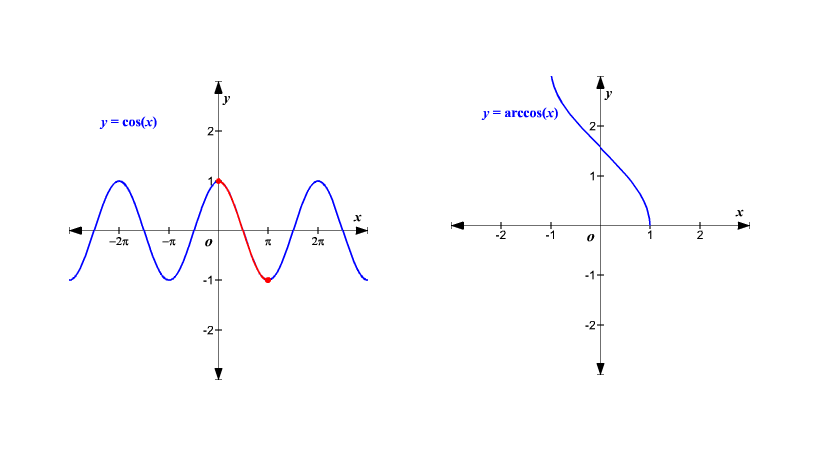
\includegraphics[width=1.2\textwidth]{Images/relation.png}
        \caption{Graphs for Cosine and Inverse Cosine Functions }
        \label{fig:Speed vs. Torque from Pittman}
    \end{figure}
    {\subsection{Characteristics of inverse function}}
    \justify
    \begin{enumerate}
        \item  The inverse function $cos^-1$ x has a 3 branch points: x=$\pm $1 , x=$\infty$
        \item It is a single value function and continuous on the interval (-$\infty$,1] and from below on the interval [1,$\infty$].
        \item Function is neither even nor odd.
        \item It is an analytic function of x and can be defined over complex numbers.
    \end{enumerate}
    \section{Requirements}
    This document is intended to represent the functional requirements for the $y = cos^-1$ function.
    Functional requirements shall be indicated by the letter "F" for the sake of simplicity, and non-functional requirements by the letter "NF". All requirements will be met with version 1.0.
    Following are the requirements needed to perform the function:
    \subsection*{List of Requirements}
    \begin{itemize}
        \item ID: FR1\\
        Owner: Pravallika Basam\\
        Version: 1.0\\
        Description: If the value of x is greater than 1 or less than -1. System should display an error. \\
        Rationale: arccos function is defined on the domain [-1,1] \\
        \item ID: FR2\\
        Owner: Pravallika Basam\\
        Version: 1.0\\
        Description: If the function has an inverse that is also a function, then there can only be one y for every x.\\
        Rationale: The function is continuous on the interval (-$\infty$,1] and from below on the interval [1,$\infty$].\\
        \item ID: FR3\\
        Owner: Pravallika Basam\\
        Version: 1.0\\
        Description: The 1st quadrant will always include the positive values whereas the {$2^n^d$} quadrant will always contain the negative values.\\
        Rationale: The principal value range of the function is [0,$\pi$].\\
        \item ID: FR4\\
        Owner: Pravallika Basam\\
        Version: 1.0\\
        Description: The type of the input data should always be double. An exception would be thrown for any other data type.\\
        Rationale:  arccos function is defined on the domain [-1,1]\\
        \item ID: FR5\\
        Owner: Pravallika Basam\\
        Version: 1.0\\
        Description: The system should produce accurate results in 1 second.\\
        Rationale: The algorithm ought to be quick enough to produce the right results.\\
        \item ID: FR6\\
        Owner: Pravallika Basam\\
        Version: 1.0\\
        Description: The value for $cos^-1(1/x)= sec^-1(x)$\\
        Rationale: The function should satisfy other related trigonometric functions.\\
        \item ID: FR7\\
        Owner: Pravallika Basam\\
        Version: 1.0\\
        Description: The value for $cos^-1(x)= \pi- sin^-1(x) $\\
        Rationale: The function should satisfy other related trigonometric functions.\\
        \item ID: FR8\\
        Owner: Pravallika Basam\\
        Version: 1.0\\
        Description: The value for $cos^-1(-x)= \pi- cos^-1(x) $\\
        Rationale: The function should satisfy other related trigonometric functions.
    \end{itemize}
    \section{PseudoCode}
    \noindent The inverse of a given number x is the inverse of the cosine function at an angle $\theta$. The arccos function can be calculated in a variety of ways. The function can be solved using following methods:
    \begin{itemize}
        \item Maclaurin's Series.
        \item Taylor's Series.
        \item Recursion
    \end{itemize}
    The Maclaurin's Series and Taylor's series are represented for the inverse cosine function as,
    \par
    $sin^-1(x) = x+\frac{1}{2} \frac{x^3}{3}+ \frac{1}{2} \frac{3}{4} \frac{x^5}{5}+\frac{1}{2}\frac{3}{4} \frac{5}{6} \frac{x^7}{7}+...$ $|x|<1$
    \par
    $cos^-1(x) = \frac{\pi}{2}- sin^-1(x)$
    \par
    = $\frac{\pi}{2}-  x+\frac{1}{2} \frac{x^3}{3}+ \frac{1}{2} \frac{3}{4} \frac{x^5}{5}+\frac{1}{2}\frac{3}{4} \frac{5}{6} \frac{x^7}{7}+...$\\[0.2 cm]
    Taylor's series is used to compute arccos due to its simplicity. This series can also be used to solve complex arguments.
    \begin{algorithm}
        \footnotesize
        \caption{Calculate arccos function}
        \begin{algorithmic}[1]
            \Procedure {Fact}{$c$}
                \State $factorial \leftarrow 1$
                \For {$i \leftarrow 1, exponent$}
                    \State $factorial \leftarrow factorial * i$
                \EndFor
                \State \textbf{return} $factorial$\
            \EndProcedure
            \Statex
            \Procedure {CalculateArccos}{$x$, $n$}
                \State $pi \leftarrow 3.14$
                \State $i \leftarrow (value-1) / (value+1)$
                \For {$i \leftarrow 1, \infty$}
                    \State $factorial \leftarrow (factorial * i)$
                    \State $sum \leftarrow pow(x,i) \Call{fact(i)} $
                \EndFor
                \State $approx\leftarrow 1+value$\
                \State $z\leftarrow (pi/2)-approx$
            \EndProcedure
            \Statex
            \State $ a \leftarrow \Call{CalculateNaturalLog}{x}$\Comment{Calculates $ln x$}
            \State $ b \leftarrow \Call{CalculateNaturalLog}{b}$\Comment{Calculates $ln b$}
            \State $result \leftarrow a/b $\Comment{Final result of $log_b x$}
        \end{algorithmic}
    \end{algorithm}
    \\[0.2 cm]
    \section{Pros and Cons of Taylor’s Series}
    \textbf{Pros}
    \begin{itemize}
        \item The simplicity of Taylor's series is its main advantage.
        \item The most difficult problems can often be solved with the help of this series.
        \item The Taylor's series is useful in creating the foundation for numerous functions and procedures.
        \item Additionally, Taylor's series helps in obtaining theoretical error boundaries.
    \end{itemize}
    \textbf{Cons}
    \begin{itemize}
        \item The time required to solve the equations is its main drawback.
        \item In Taylor's series, the round-off error and truncation error might come that disturbs the whole calculation.
        \item It is not as efficient when comes to direct approximation.
    \end{itemize}
    \section{Working of the Function}
    \begin{figure}[hbt!]
        \centering
        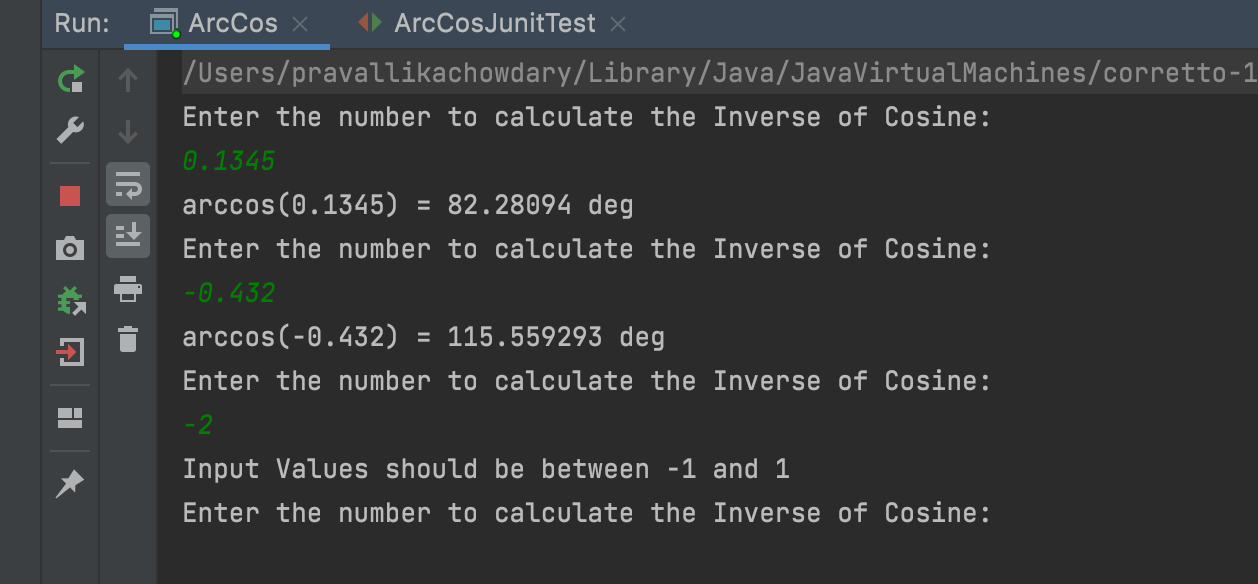
\includegraphics[width=1.2\textwidth]{Images/JavaImplementation.png}
        \caption{Text-based user interface of the arccos implementation}
        \label{fig:Speed vs. Torque from Pittman}
    \end{figure}
    \par
    Java is used for the arccos function implementation. The IDE used to develop code and test cases is called Intellij. And, The type of interface is a text-based user interface (TUI).
    \section{Debugger}
    \subsection{Description}
    IntelliJ IDEA provides a debugger for Java code. Run your software while it is connected to the debugger during a debugging session. The debugger's will then interrupt the execution of the programme and give you details about what's going on internally at each step. This makes it easier to find and correct errors in the program.
    \begin{figure}[hbt!]
        \centering
        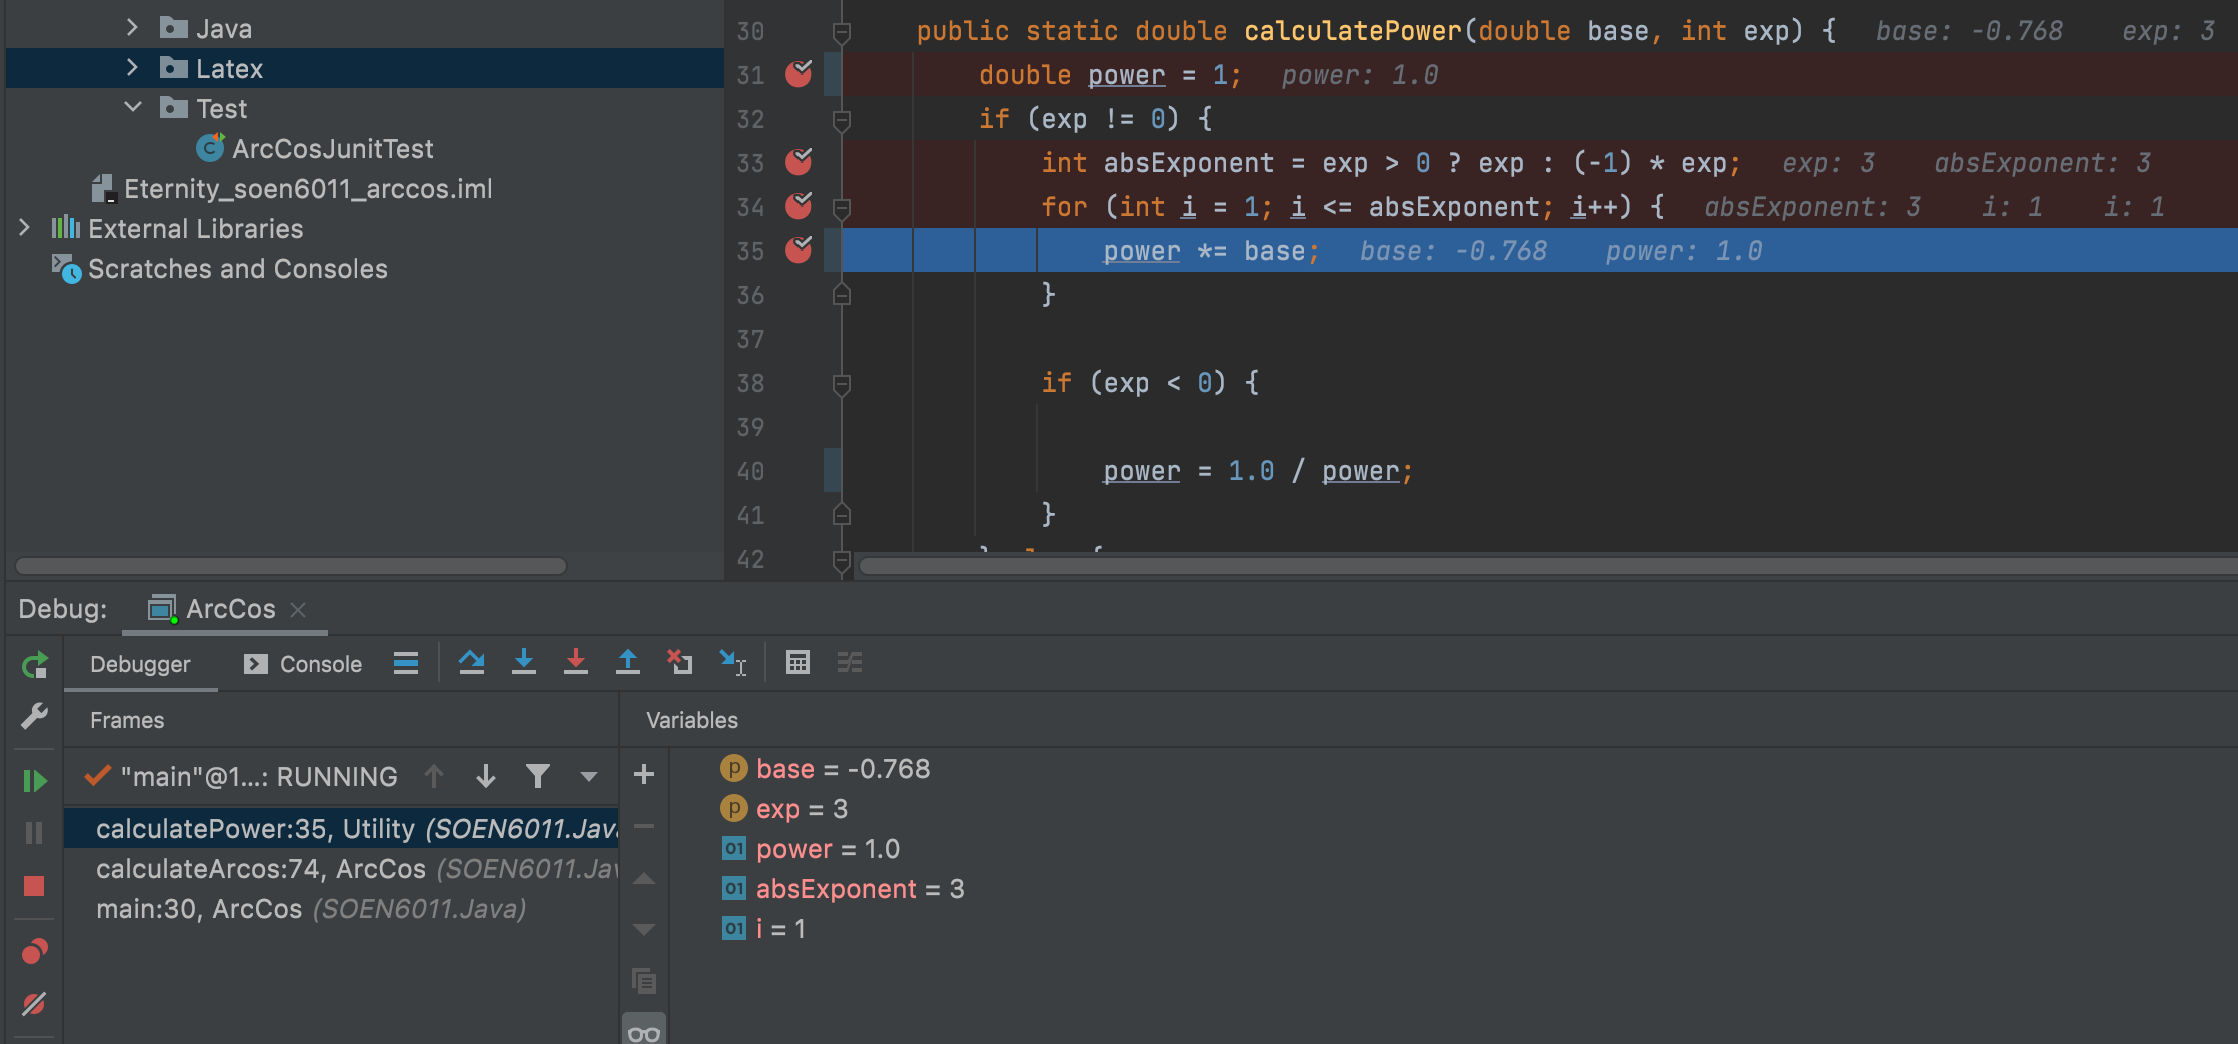
\includegraphics[width=5.0in,height=3.0in]{Images/Debugger.png}
        \caption{Working of an IntelliJ Debugger}
        \label{fig:Speed vs. Torque from Pittman}
    \end{figure}
    \subsection{Pros}
    \begin{itemize}
        \item Debugging mode makes it incredibly simple to test predicted outputs as variables' values can be changed instantly.
        \item It can step into or over a statement using step filtering technique.
        \item It offers event-based breakpoints.
        \item It offers a feature that shows the item's logical structure, enabling us to comprehend the object in a meaningful structure or view.
    \end{itemize}
    \subsection{Cons}
    \begin{itemize}
        \item The JVM design will cause method breakpoints to significantly slow down the debugger. The overall performance may even be slowed down as a result of this.
        \item When the number of breakpoints is high, the debugger may crash.
    \end{itemize}
    \section{Quality Attributes}
    \subsection{Correctness}
    The function is checked against all potential values of x , and the outcomes are confirmed using a real scientific calculator.
    \subsection{Efficient}
    The program is designed to produce output quickly, perhaps in less than a second. Additionally, the program is space-efficient as less memory is utilised to store the variables.
    \subsection{Maintainable}
    Since the program is divided into methods for performing different functions, adding new functionality or making changes is made simpler. Any developer may easily understand the code by reading the comments and the documentation.
    \subsection{Robust}
    In order to prevent software failure, the application is tested for every possible type of incorrect input.
    \subsection{Usable}
    Since the program uses a textual interface, which is more practical and understandable, anyone may do the task effectively.
    \section{Quality of Source Code}
    \subsection{Description}
    To evaluate the quality of source code, SonarLint is used. As you code, this IntelliJ IDE addon helps you find and resolve quality and security issues. Similar to a spell checker, SonarLint highlights errors while offering immediate feedback and detailed remedial instructions to produce clean code instantly.
    \subsection{Advantages}
    \begin{itemize}
        \item Highly configurable and supports any coding standard.
        \item It highlights source code that is not reachable.
        \item It provides the appropriate error/warning messages as per the coding style applied.
    \end{itemize}
    \subsection{Disadvantages}
    \begin{itemize}
        \item SonarLint does not support viewing your code coverage in IntelliJ.
        \item There is no mechanism to report concerns with sonarlint.
    \end{itemize}

    \begin{thebibliography}{9}
        \bibitem{Checkstyle}
        Checkstyle,
        \\\texttt{https://checkstyle.sourceforge.io/}

        \bibitem{Eclipse}
        Debugger,
        \\\texttt{https://www.eclipse.org/}

        \bibitem{Style}
        Google programming style,
        \\\texttt{https://google.github.io/styleguide/javaguide.html}

    \end{thebibliography}
    \section{References:}
    \begin{enumerate}
        \item An excellent reference book for Taylor series of functions and many other
        properties of mathematical functions can be found in Milton Abramowitz and
        Irene A. Stegun, Handbook of Mathematical Functions (Dover Publications, Inc.,
        New York, 1965). This resource is available free on the web and can be either
        viewed or downloaded from \\http://people.math.sfu.ca/~cbm/aands/.
        \item Recently, a new reference that aims to update the classic reference book of
        Abramowitz and Stegun (see Ref. 1) has been published. The NIST Handbook of
        Mathematical Functions, edited by Frank W.J. Olver, Daniel W. Lozier, Ronald
        F. Boisvert and Charles W. Clark (Cambridge University Press, Cambridge, UK,
        2010) has become an instant success! An electronic form of this book is available
        free on the web and can be viewed from http://dlmf.nist.gov/.
        \item https://byjus.com/maths/inverse-trigonometric-functions
    \end{enumerate}
\end{document}
